\chapter{Introduction}
\label{ch:intro:intro}

For humans and other animals, in any given context, an adaptive behavior is defined as the capacity to execute the action that will maximize immediate or future rewards, while minimizing energetic expenditure.
For example, consider any solitary hunter that would wait for the right time to attack: 
    when the prey is most distracted or vulnerable.
However, in some situations, the appearance of a sensory cue will not only indicate which action should be performed, but also how long, after appearance of the cue, this action must be initiated~\cite{Balsam2009Map, Nobre2018NatRevNeurosci}.
For instance, athletes performing sprint races learn by experience that the \textit{go} command, signalling them to start running, will be given in two seconds after the \textit{set} command.
False starts, i.e., beginning to run too early, demonstrates athletes' accurate estimation of the 2 second interval between the \textit{set} and \textit{go} commands.
More generally, the ability of animals to exploit temporal regularities in nature is crucial for survival:
    The appearance of a sensory cue at a given time can predict food availability, predator attack, or mating opportunity~\cite{Kacelnik2002,Gallistel1990book}.
\par
In this chapter, first I discuss two possible mechanisms that could give rise to the perception of elapsed time.
Then, I will present some evidence of how these mechanisms are implemented, in particular,  the role of a certain brain structure that is implicated by both of the above mechanisms, however, in different ways.
Finally, I will lay out the question and the hypothesis underlying this work and the structure of the following chapters.

\section{Internal Time Estimation}
\label{ch:intro:InternalTimeEstimation}

Understanding how animals adapt their behavior to time intervals of various durations is challenging, because unlike sensory modalities (vision, olfaction, audition), time is not a material entity and animals are not equipped with a sense organ for time perception.
Time perception in the timescale of a few seconds (compared to, say, 100~ms) seems to be even more puzzling, since it is much longer than intrinsic properties of neural function~\cite{Buhusi2005NatRevNeuro}.
\par
One influential idea in the field of systems neuroscience, hereafter referred to as the \emph{internal clock}\!, posits that complex nervous systems have acquired the ability to estimate elapsed time and use this representation to determine if the duration of a given time interval is similar to (or different from) a previously learned interval~\cite{Gibbon1977, Miali1989NeuComp, Gouvea2015Elife,Wittmann2013NatRevNeurosci}.
Irrespective of its exact neural implementation, which will be discussed \hyperref[ch:intro:BGTime]{later}, the internal clock works according to the following principle.
Once a cue appears to signal the beginning of a time interval (e.g., the \textit{set} command in sprint races), the neuronal time quanta begin to accumulate.
Time interval estimation consists in comparing the magnitude of this ongoing accumulatory process with a stored value determined through experience (e.g., multiple exposures to time intervals between \textit{set} and \textit{go} commands in sprint races)~\cite{Simen2011JNeuro}.
Errors in counting neuronal time quanta will accumulate with time too.
Consequently, such a mechanism predicts that time estimation accuracy should degrade proportionally to the duration of the time interval, which has been verified in humans and animals~\cite{Gibbon1977, Lejeune1991LearnMotiv, Rakitin1998, Whitaker2003JExpPsy, Zarco2009JNeurophys, Hinton2004, JazayeriNN2018, Gallistel2004}.
This is a feature of timing, generally referred to as the \emph{scalar property}\!, and resembles the Weber's law in sensory perception.\footnotemark
\footnotetext{
    ``Formulated by Ernst Weber in 1831 to explain the relationship between the physical intensity of a stimulus and the sensory experience that it causes.
    Weber’s Law states that the increase in a stimulus needed to produce a just-noticeable difference is constant.
    Later, Gustav Fechner (1801-1887) generalized Weber's law by proposing that sensation increases as the logarithm of stimulus intensity: $S = k logI$, where $S=$ subjective experience, $I=$ physical intensity, and $k =$ constant.''~\cite{Buhusi2005NatRevNeuro}
    }
\par
Another proposal suggests that time estimation ultimately relies on task-specific emergent properties of interacting neuronal networks, rather than a pure time-dedicated internal clock~\cite{Paton2018NeuronRev}.
Such an \emph{emergent}\! clock also has the assumption that the origin of time perception is internal, i.e, organisms infer the elapsed time purely from their neuronal dynamics.

\subsection{Central Clock}
\label{ch:intro:InternalTimeEstimation:Central}

It has been long proposed that a central clock provides temporal information for organisms~\cite{gibbon1984AnnalsNYAS, Killeen1988}.
The \emph{pacemaker-accumulator}\! model is the most prominent computational account of such a central clock.
In essence, this model postulates:
    a pacemaker, which generates periodic pulses at intervals shorter than those being estimated;
    a switch, that following training, gates pulses through for a certain duration;
    an accumulator, downstream of the switch, that records the number of pulses in working memory;
    a reference memory, that holds the number of pulses that previously have been reinforced;
    a comparator, which determines whether the accumulated value is close enough to the reference value to warrant a response or not~\cite{gibbon1984AnnalsNYAS}.
This model explains the scalar property by introducing sources of variability to its components.
The pacemaker-accumulator model has many advantages:
    it is very straightforward, intuitive, and biologically feasible;
    it has clear separation of memory and decision-making systems, which could map to neural structures;
    and it is extremely successful in predicting behavioral data, given its simplicity~\cite{Buhusi2005NatRevNeuro}.
\par
Other internally-driven models of temporal processing have been proposed as well.
The \emph{Beat-frequency model}\! is another dedicated model for interval timing~\cite{Paton2018NeuronRev}.
In this model, different intervals could be decoded from a bank of oscillators with different frequencies, since subgroups of such oscillators may be in the same phase at intervals much greater than those of individual oscillators.
For example, three oscillators with periods of~5,~8, and~11~s are in the same phase every 440~s.\footnotemark\
\footnotetext{
    Mathematically, for any number of oscillators, it will be their \textit{least common multiple}.
    }
Hence, by choosing various subgroups and detecting the time at which they are phase-locked, one could generate a wide range of intervals.
This model is also biologically feasible, as each oscillator could be as simple as a single neuron with a constant firing rate.
Consider a series of these \textit{oscillatory} neurons being reset with the stimulus (at the beginning of the interval).
At any point in time, their spiking could be observed by a downstream structure.
A subset of these neurons that fire at the time of reinforcement (i.e., the end of the interval) could represent a neural code for this particular interval~\cite{Matell2004CogBrainRes}.
Similarly, other subsets could encode different intervals.
Among others, \Citeauthor{Miali1989NeuComp} simulated the beat-frequency model with 500 units oscillating at~5 to~15~Hz~\cite{Miali1989NeuComp}.
One output unit received single synapses from every oscillatory unit and the strength of each synapse followed a simplified Hebbian rule.
This model managed to learn to encode intervals ranging from 200~ms to 10~s.
\par
Finally, another class of models are based on ramping activity of neurons.
These models propose that a linear metric of elapsed time is encoded in decreasing/increasing firing rate of neurons~\cite{Paton2018NeuronRev}.
Crucially, the slope of the ramping must correlate negatively with the duration of the interval, since the maximum possible firing rate is relatively constant~\cite{Jazayeri2015CurrBiol}.
Moreover, neurons have timescales of tens of milliseconds, thus, for these model to account for time estimation in behaviorally-relevant timescales, i,e., several hundreds of milliseconds to seconds, there must be a feedback mechanism.
Simulations by \citeauthor{Gavornik20009PNAS} demonstrate that recurrent excitatory synapses could provide such a feedback signal~\cite{Gavornik20009PNAS}.
In this network, the activity of each neuron, if isolated, would decay after stimulus presentation.
However, by introducing recurrent connections, lateral propagation of activity in the network decreases decay rate of each neuron's activity in response to a stimulus.
In other words, the network modifies the temporal properties of the response of individual neurons, which could translate to elapsed time representation.

\subsection{Emergent Clock}
\label{ch:intro:InternalTimeEstimation:Emergent}

A different class of models postulate that representations of time emerge from distributed dynamics of neural networks.
These models differ from those discussed in \autoref{ch:intro:InternalTimeEstimation:Central} in that these models are not localized, i.e., they could involve different brain areas however, they similarly assume time estimation is internally driven.
These models assume that sensory, motor, and cognitive systems that are not specifically dedicated to timing might form networks that (after training) act as interval timers~\cite{Wittmann2013NatRevNeurosci}.
\par
One type of such models, namely state-dependent networks, proposes that neural networks inherently contain temporal information as a result of their complexity.
In a seminal work, \citeauthor{Karmarkar2007Neuron} simulated a network of 400 excitatory and 100 inhibitory neurons, recurrently connected and exhibiting synaptic plasticity~\cite{Karmarkar2007Neuron}.
This network was then exposed to two identical events, 100~ms apart (e.g., two auditory tones).
Due to complex synaptic processes, the state of the network at any point in time after the presentation of the first stimulus was unique.
Thus, the population response to the second stimulus inherently encoded the duration between the two stimuli.
In this fashion, various intervals could be decoded from dynamics of ever more complex networks.
Indeed, in a more recent work, \citeauthor{Perez2018JNeurosci} simulated a recurrent network of 800 excitatory and 200 inhibitory neurons~\cite{Perez2018JNeurosci}.
The neurons were randomly connected and received two membrane currents induced by the stimulus (one inhibitory, one excitatory).
In addition, each neuron in the network also received two recurrent inputs.
All of the synaptic currents followed time-varying dynamics.
These temporal synaptic properties (such as time constant of neurotransmitter release, inhibitory input current dynamics,~\ldots) allowed an optimal Bayesian decoder to produce interval-selective responses, in the range of several hundred milliseconds.
This network, given parameter values within physiological range, could demonstrate scalar property as well.
\par
This, by no means, is a comprehensive review of all the literature on timing models and that is not the focus of this manuscript.
There are numerous articles proposing different neurocomputational models (using ramping activity, drift diffusion, synfire chain, coincidence detector,~\ldots) to account for psychophysical evidence of timing behavior in humans and other animals.
\Citeauthor{Paton2018NeuronRev} reviewed many of these models in a recent paper~\cite{Paton2018NeuronRev}.
\section{Embodiment}
\label{ch:intro:Embodiment}
\epigraph{Je pense, donc je suis (I think, therefore I am).}
{\textit{ Ren\'{e} Descartes, Discours de la M\'{e}thode}}
\noindent
I am not invoking Descartes just because I am in France, there is a point too!
This quote implies a duality between the brain and the body: the reason I exist is my mind, not the body.
Although the delicacies of the \emph{mind-body problem} is out the scope of this work, a simple reading suggests that the brain is the ruler of the body.
This simple unidirectional approach has been vastly used in fields such as robotics, by designing agents with a central processing unit that commands the actuators.
This simplicity, however, comes at a cost.
The most unremarkable actions that animals perform with little cognitive load, such as grasping an object or locomotion, have proved to be painstakingly difficult to implement in robots~\cite{Pfeifer2006Book}.
For decades now, an alternative approach has been proposed that has improved the performance of robotic agents~\cite{Brooks1991AI}.
\par
Since then, embodiment, has enabled engineering of more robust and adaptable robots, inspired from biological organisms.
\citeauthor{Pfeifer2007Sci} present insect locomotion as a very convincing example of taking advantage of embodiment principles in robotics.
Insects demonstrate coordinated walking and running, which given their six legs, pose a challenging problem with dozens of degrees of freedom, in particular on uneven terrains.
It is plausible to assume they do not solve the inverse kinematic problem for all their joints at all the times, which was the classic approach in robotics and requires enormous computational resources.
However, by taking embodiment into account, pushing back a single leg, which could be detected by angle sensors in the joint, could command all the other joints to move in the ``correct" direction.
This way, a low level communication between the legs could be exploited to achieve leg coordination without any central controller in the nervous system~\cite{Pfeifer2007Sci}.
\par
In the animal kingdom, embodiment enables both cognition--even the most abstract processes, like mathematical reasoning~\cite{Lakoff2000Book}-- and action.
In this framework, behavior is not reduced to internal computations, rather it is the manifestation of intricate brain-body-environment interactions.
Perception of the external world relies upon how the information is channeled through different parts of the body and differences in the shape of body parts alters the incoming and outgoing signals~\cite{Gomez2019Neuron}.
The body also shapes the way we interact with our environment.
\Citeauthor{Gomez2019Neuron} discuss the interesting case of the well-coordinated stepping behavior in human infants~\cite{Gomez2019Neuron}.
When held upright, newborns show coordinated step-like movements.
This phenomenon disappears after around~2~months.
While it was long assumed that this is due to developing nervous system, \citeauthor{Thelen1984InfBeh} showed that loss of stepping behavior is due to weight gain of the legs and it can be recovered by submerging the legs in water (which would decrease their mass)~\cite{Thelen1984InfBeh}.
Thus, embodiment, through brain-body-environment interactions subjects us to the laws of physics---having to deal with gravity, friction, and most relevant to this work, forward arrow of time~\cite{Pfeifer2006Book}.


\subsection{Embodied Clock}
\label{ch:intro:Embodiment:Embodied Clock}
\epigraph{Time by itself does not exist\ldots It must not be claimed that anyone can sense time apart from the movement of things.}
{\textit{Lucretius, Book 1}}
\noindent
Principles of embodiment could be applied to time-estimation problems as well.
All the sensorimotor processes that comprise embodiment (and indeed everything else!) unfold in time.
Especially, movement has long been associated with time estimation, as far as one study stating that ``timing is inexorably tied to movement"~\cite{Wiener2019eNeuro}.
\par
As early as \citeyear{Skinner1948}, it has been reported that periodic reward delivery leads to `superstitious' behavior, i.e., performing stereotypical actions between consecutive deliveries of the reinforcer~\cite{Skinner1948}.
For example, one pigeon was conditioned to turn counter-clockwise in the cage two or three times between each reward delivery which was every 5~s, irrespective of the animal's behavior.
Each pigeon in this study developed such a unique behavior~\cite{Skinner1948}.
Similar phenomenon has been reported in many other species as well.
\Citeauthor{Wilson1953} trained rats to press a lever after progressively longer intervals (from 15~s to 30~s) to get a food pellet~\cite{Wilson1953}.
Rats slowly adjusted their lever presses to the scheduled interval, however, during the interval, they too engaged in a recognizable chain of behaviors that the authors called `collateral'.
These behaviors were also unique to each animal.
Interestingly, with increasing the interval between reward deliveries, more links were added to the chain of collateral behaviors~\cite{Wilson1953}.
Both studies mentioned above explain these behaviors as being accidentally reinforced by reward delivery, which would make them more probable to occur later, which in turn would strengthen their association with the reward~\cite{Killeen1988}.
Such a mechanism explains why these behaviors are unique to individual subjects.
Developing accidentally-reinforced behaviors could bring about repercussions.
\Citeauthor{Falk1971}, in a very enlightening article, discusses `adjunctive' behavior in food-deprived rats without any water deprivation~\cite{Falk1971}.
When exposed to intermittent food delivery during their daily test session (3~hr long), animals followed each food pellet intake with consumption of excessive amounts of water (up to half their body weight during the session) until the next food delivery, while almost no water was consumed during the rest of the day, despite being available ad libitum.
This form of adjunctive behavior persisted even after water consumption during the session was discouraged by punishment~\cite{Falk1971}.\footnotemark
\footnotetext{
    He then discusses that even though this behavior seems absurd (``heating a large quantity of room-temperature water to body heat and expelling it as copious urine is wasteful for an animal already pressed for energy stores by food deprivation"), in certain ecological settings, it might provide an adaptive response even with evolutionary advantages.
    }
\par
Modern technology has enabled synchronized video tracking of behaving animals.
In tasks in which reinforcement is contingent upon respecting time intervals, animals do not stay still, but they take advantage of the structure of their environment to develop stereotyped motor routines whose duration amounts to the temporal constraint of the task.
In one study, rats and pigeons, trained to discriminate 12~s stimulus from 6~s, developed `collateral' behaviors.
Rats, during the stimulus, engaged in sniffing, rearing, grooming, and moving from one lever to another.
Similarly, birds displayed pecking, bobbing\footnotemark, wing flapping, and moving between the keys in their cage.
Quantifying these behaviors better predicted their temporal judgement than the passage of time~\cite{Fetterman1998BehProc}.
\footnotetext{
    For those unfamiliar with bird behavior (such as myself), \emph{bobbing} refers to the two-phase movement of the head in birds, most commonly seen during walking when they hold their head while moving the body forward and then thrust their head faster than their body.
    Watching youtube clips is advised!
    }
In one of the rare studies with precise monitoring of behavior, \citeauthor{Gouvea2014} trained rats (and one mouse) to categorize an interval as shorter or longer than 1.5~s by pressing a lever correspondingly.
Animals demonstrate highly stereotyped and idiosyncratic behavior during the interval.
Critically, their perceptual report was predicted based on their behavior, even from early in the trial~\cite{Gouvea2014}.
Similar idiosyncratic embodied strategies were also used by rats trained to reproduce a 700~ms interval by waiting between successive lever presses.
\Citeauthor{Kawai2015} reported that animals developed very specific and reproducible limb movements to fill the required interval~\cite{Kawai2015}.
Earlier article from our lab...
\par
Humans, too, seem to resort to motor activity to estimate time.
Naturally, people tend to develop rhythmical movements of body parts (e.g., tapping fingers or feet, moving arms, and nodding heads) to perceive elapsed time~\cite{Merchant2016CurrOp}.
Similarly, humans, as young as 7~years old, estimate suprasecond time intervals by counting~\cite{Wilkening1987, Rakitin1998}.
Although counting could be in their heads (i.e., not out loud), it is difficult to separate it from the repeated experiences of counting the passing seconds aloud in everyday life, which is a motor activity:
    a sequence of coordinated movements across respiratory, laryngeal and supraglottal articulatory systems.
Around 97\% of adults default to counting as a time estimation strategy, and interestingly, in research, different sorts of measures has been employed to prevent use of counting in favor of a more \textit{pure} time estimation strategy~\cite{Rattat2012}.\footnotemark
\footnotetext{
    It is noteworthy that the devices we use to measure time mostly do so by moving objects in space. Also, we extensively use metaphors containing movement and space references when speaking of time (\textit{holidays are approaching}, \textit{time flies})~\cite{Winter2015Cortex}. 
    }
There is convincing evidence of beneficial impact of movement in time estimation.
Instructing human subjects to not use motor strategies, or otherwise interfering with overt movements, lowers their performance in a variety of time estimation tasks~\cite{Morillon2017PNAS, Wiener2019eNeuro, Meegan2000, Rakitin1998, Fautrelle2015PlosOne, Monier2019DevSci}.










\subsection{Cost}
\label{ch:intro:Embodiment:cost}



% There is convincing experimental evidence that our perception of time is not isomorphic with the time measured by human-made clocks and strongly depends on contextual factors affecting the subjects' attentional, motivational or emotional state~\cite{Paton2016Sci, Coull2004Sci, Droit2007TICS, Effron2006Emotion, Pariyadath2007Plos, Gable2012PsychSci}.\footnotemark
% \footnotetext{
%     Time flies when we are fully engaged in an activity (giving a 20 minutes-long neuroscience talk) but can terribly drag when we are bored (listening to a 20 minutes-long neuroscience talk).
%     }
% Both emergent and dedicated algorithms for time estimation account for the state-dependant variance in time perception by a neuromodulator-based slowing or speeding of neuronal clocks~\cite{Paton2016Sci, Simen2016Sci}.
% Alternatively, the strong influence of contextual factors on time perception may indicate that mechanisms beyond internal neural activity play a primary role in how humans and animals perceive time and adapt their behavior accordingly.
% Indeed, the embodiment framework proposes that important aspects of cognition are determined by physical features of the body, which in turn influence how humans or animals interact with their environment~\cite{Pfeifer2006Book}.
% That is to say, animals (and humans) may primarily replace the abstract concept of having to estimate a certain duration with an embodied strategy that happens to last the same duration.
% In tasks whereby a fixed time interval must be respected to obtain a reward, animals do not stay immobile, rather they take advantage of the structure of their environment to develop ritualistic motor routines whose durations match these task-specific temporal constraints~\cite{Gouvea2014, Kawai2015, Rueda2015NN}.
% Although humans can seemingly estimate time, either by counting in their heads or otherwise, it is difficult to separate this mental faculty from memories of counting the passing seconds aloud, which in turn is a sequence of coordinated movements across respiratory, laryngeal and supraglottal articulatory systems, or in general, any motor memory~\cite{Coull2018}.
% In addition, humans naturally tend to estimate time intervals through rhythmical movements of some of their body parts (by flicking fingers, moving arms, nodding heads or tapping feet).\footnotemark
% \footnotetext{
%     It is noteworthy that, to reliably estimate time, humans have created clocks, that indicate time by moving objects in space and extensively use metaphors containing movement and space references when speaking of time (\emph{holidays are approaching}, \emph{time flies})~\cite{Nunez2013TICS,Winter2015Cortex}.
%     }
% It has also been recently argued that explicit perception of time may be constructed implicitly through association between the duration of an interval and its sensorimotor content~\cite{Coull2018}.
% Thus, animals (and humans) may primarily rely on the movement of their body in space to estimate time~\cite{VoletRev2013}, which incidentally explains why brain regions involved in movement control, such as the \gls{bg}, have consistently been associated with time perception~\cite{Coull2018}. 








\section{Implementation}
\label{ch:intro:implementation}
% why basal ganglia
% (maybe first the anatomy)
The renowned neuroscientist, David Marr (1945--1980), proposed three levels of analysis to understand a complex system.
First, the \emph{computational level}, describes the task and the goal that need be achieved.
Second, the \emph{algorithmic level}, specifies the procedures for manipulating the information associated with the computation.
Third, the \emph{implementation level}, characterizes how to physically realize the algorithm~\cite{Willshaw2015Marr}.
\Citeauthor{Krakauer2017Neuron} in a perspective article that greatly influenced this work, present the following example~\cite{Krakauer2017Neuron}.
Understanding a flying bird could be achieved at three levels:
A bird attempts to \textit{fly} (level~1:~computation) by \textit{flapping} its wings (level~2:~algorithm) which is plausible due to aerodynamic properties of the \textit{feathers} (level~3:~implementation).
They then argue that the explanatory power of studying feathers alone is fundamentally restricted, evident by some birds that fly without feathers and some types of flight that does not require flapping.
As it pertains to the link between brain and behavior, it may be much more difficult to infer the algorithms used by brain from studying the nervous system, compared to understanding them at a computational level.
\par
Thus far, I portrayed the case for behavioral importance of time estimation (level~1), and different possible strategies to estimate an interval (dedicated, emergent, and embodied clock, level~2).
In this section, I will address how those strategies could be implemented in the brain (level~3).
Of all the brain regions that have been suggested to be involved in time perception\footnotemark, across a wide range of tasks and scales, \gls{bg} is of unique interest.
\footnotetext{
    So many brain structures have been found implicated in time estimation that prompted \citeauthor{Wittmann2013NatRevNeurosci} to state: ``one may be inclined to state that researchers are actually clueless concerning the question of how the brain processes time."~\cite{Wittmann2013NatRevNeurosci}.
    }
For decades, \gls{bg} have been the focus of many timing studies~\cite[see][]{Paton2018NeuronRev}, as well as motor studies~\cite[see][]{Turner2010CurrOpinNeurobiol}.
Therefore, it could be considered as an ideal candidate structure to mediate timing behavior through sensorimotor mechanisms.

%===========================================================
\subsection{The Basal Ganglia}
\label{intro:BGAnatomy}
The \glsentrylong{bg} are a set of interconnected subcortical nuclei.
Their neural organization, cell types, and neurochemical markers are highly conserved in vertebrates for over 500 million years, ranging from the lamprey to the primates~\cite{Grillner2016BG}.
The \gls{bg} may be viewed as a two-input two-output system.
The striatum and the \gls{stn} are the input structures receiving excitatory afferents from virtually the entire cerebral cortex and thalamus.
In rats, compared to \gls{stn}, the striatum contains more than two-hundred times more neurons and thus is regarded as the main input to the \gls{bg}~\cite{Oorschot1996}.
\par
The output nuclei are the internal segment of the globus pallidus, i.e., \gls{gpi}, and the \gls{snr}.
They are exclusively composed of GABAergic projection neurons with high baseline firing rates.
\Gls{gpi} and \gls{snr} hold the targeted premotor centers in the brainstem and thalamus under tonic inhibition~\cite{Redgrave2010}.
There are no direct connections from the \gls{bg} efferents to motor neurons of the brainstem or spinal cord~\cite{Mink1996}.
\par
Other than the input and output nuclei, the \gls{bg} also include the external segment of the globus pallidus, i.e., \gls{gpe}, which is innervated by the striatum and the \gls{stn}.
Most neurons in the \gls{gpe} provide GABAergic projection to the \gls{stn}, \gls{gpi}, and \gls{snr}~\cite{Dudman2015Book}.
\Gls{stn} in turn innervates the \gls{gpe} and the output nuclei.
\Gls{stn} efferents form the only intrinsic excitatory connections in the \gls{bg}, an otherwise inhibition-dominated structure.
The other nuclei of the \gls{bg} are the \gls{da}-containing centers of the midbrain, namely ventral tegmental area, and \gls{snc}.
Ventral tegmental area preferentially targets the ventral striatum and \gls{snc}, projects to the dorsal striatum~\cite{Cox2019NatRevNeurosci}.
These nuclei innervate striatal neurons in a dense and rather uniform manner, however, they also target structures external to the \gls{bg}, like several cortical and limbic regions.
\autoref{fig:intro:BGAnatomy} summarizes the anatomy of the \gls{bg}.
\begin{figure}[bth]
	\begin{center}
		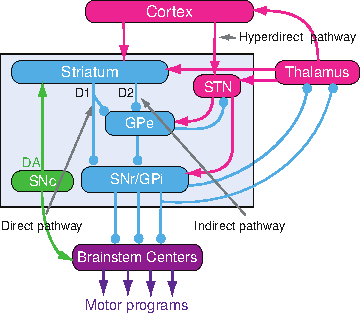
\includegraphics[width=0.7\linewidth]{ch-intro/figures/BGAnatomy}
		\caption[Anatomy of the Basal Ganglia]
		{\textbf{Schematic Anatomy of the basal ganglia.}
		The gray highlighted rectangle depicts the BG nuclei.
		Arrows show anatomical connections (\textit{red}: glutamatergic; \textit{blue}: GABAergic; \textit{green}: DAergic).
		STN:~subthalamic nucleus;
		GPe:~globus pallidus externus;
		SNc:~substantia nigra pars compacta;
		SNr:~substantia nigra pars reticulata;
		GPi:~globus pallidus internus;
		DA:~dopamine.
		Figure slightly modified from~\cite{Grillner2016BG}.
		}
		\label{fig:intro:BGAnatomy}
	\end{center}
\end{figure}

%=============================================================
\subsubsection{Striatum} \label{intro:anatomy:striatum}
%order of material: MSNs > interneurons > topography > DLS/DMS
The striatum is the main input nucleus of the \gls{bg} and one of the largest undivided structures in rodent brain atlas~\cite{Hintiryan2016NN,Hunnicutt2016}.
Despite having several cell types, GABAergic \glspl{msn} constitute~90--95\% of its neural population.
Their name stems from their morphological appearance, their size and the abundance of their dendritic processes~\cite{TURNER2000BasalFunction}.
\Glspl{msn} receive glutamatergic inputs from the entire cortex, thalamus, and amygdala.
These excitatory afferents make up 80\% of all the synapses in the striatum~\cite{Wilson2007GABAergicNeostriatum}.
Several other inputs modulate the responsiveness of the \glspl{msn} to massive excitatory synapses, namely \gls{da} afferents, inhibitory input from GABAergic interneurons (and from \gls{msn} collaterals), and input from cholinergic interneurons~\cite{Dudman2015Book}.
Consequently, \glspl{msn} are mostly quiescent, except during motor activity or in response to sensory stimuli~\cite{KandelBook2001}.
\par
Based on morphological and neurochemical identification, there are two major types of interneurons within the striatum, which make up~5--10\% of striatal neural population:
    the medium aspiny GABAergic interneurons, and the large aspiny cholinergic interneurons.
The most abundant type of GABAergic interneuron expresses parvalbumin.
Parvalbumin-positive interneurons are physiologically characterized by their hyperpolarized resting potential and fast spiking activity.
Thus, they are usually referred to as the \glspl{fsi}~\cite{Dudman2015Book}.
They target \glspl{msn} at the soma level by gap junctions and provide powerful GABAergic synapses to several hundreds of surrounding \glspl{msn}~\cite{Grillner2016BG, Gage2010FSI}.
Although they are scarce, with higher firing rate compared to \glspl{msn}, they are capable of delaying action potentials in the neighboring \glspl{msn}~\cite{Wilson2007GABAergicNeostriatum}.
\par
Large cholinergic interneurons are the other type of striatal interneurons.
Their soma could be as large as~40~$\mu$m in diameter, with expansive arborization and an axon that extends over~2~mm~\cite{Dudman2015Book}.
They have tonic discharge patterns, and in primate, are called \textit{tonically active neurons}.
\Glspl{fsi} and cholinergic interneurons are not noticeable in number, nonetheless, they are believed to strongly contribute to the dominance of inhibition in the striatum~\cite{Gage2010FSI}.
In addition to these two, several other types of interneurons within the striatum are described as well~\cite[see][]{Grillner2016BG, Dudman2015Book}.

\paragraph{Organization of Cortical Inputs}
It has been long known that corticostriatal projections are topographical, roughly following the rostro-caudal and latero-medial organization in the cerebral cortex.
For instance, frontal cortices project to rostral areas, sensorimotor cortex provides input to dorsal striatum, and parietal cortex to more caudal areas~\cite{Dudman2015Book}.
Such topographical organization suggests parallel circuits for limbic, cognitive, and sensorimotor processes via cortico-\gls{bg}-thalamo-cortical loops~\cite{Alexander1986}.
In this framework, the sensorimotor loop consists of \gls{dls}, ventrolateral thalamus, and sensorimotor cortices.
Similarly, the limbic (emotional) loop includes the ventral striatum, dorsomedial thalamus, and limbic areas (amygdala, limbic cortices, and hippocampus).
Finally, the cognitive (associative) loop comprise the \gls{dms}, anterior ventral thalamus, and frontal cortices~\cite{Jahanshahi2015NatRevNeurosci}.
However, reduced number of neurons from cortex to \gls{bg} outputs by a factor of more than one million, implies integration of information from different loops to shape the appropriate behavior~\cite{Boraud2018ProgNeurobiol}.
\par
In the dorsal striatum, loose somatotopic organization has also been long reported~\cite[see][as an early review]{Mink1996}.
In \citeyear{Carelli1991}, \citeauthor{Carelli1991} recorded from hundreds of neurons during movement and somatosensory stimulation.
They found that more than 70\% of recorded neurons in the \gls{dls} responded to movement, passive manipulation or cutaneous stimulation.
Moreover, neurons selective for an individual body part (e.g., forelimb, neck, snout,\dots) were generally located in close proximity, generating a somatotopic map~\cite{Carelli1991}.
Such an anatomical mapping from sensorimotor cortices to \gls{dls} has recently been quantitatively scrutinized in mice~\cite{Hunnicutt2016, Hintiryan2016NN}.
These studies, using multiple injections of anterograde tracers, constructed a comprehensive excitatory input map of the dorsal striatum.
\autoref{fig:intro:InputMap} shows an example of different cortical regions projecting to the \gls{dls} in a somatotopic manner.
Interestingly, cluster analysis of cortical regions projecting to arbitrarily-defined striatal voxels revealed dorsal striatal subregions which relatively agreed with parallel circuits for limbic, cognitive, and sensorimotor processes.
With the strictest clustering criteria, \citeauthor{Hunnicutt2016} identified two areas, which map roughly to the \gls{dls} and \gls{dms}\footnotemark~\cite{Hunnicutt2016}.
\footnotetext{
    \Gls{dls} and \gls{dms} correspond to the putamen and caudate nuclei, respectively.
    In primates, the internal capsule divides the striatum in two halves, thus the use of caudate-putamen nucleus instead of the striatum is more common.
    }
\begin{figure}[bth!]
  \begin{center}
    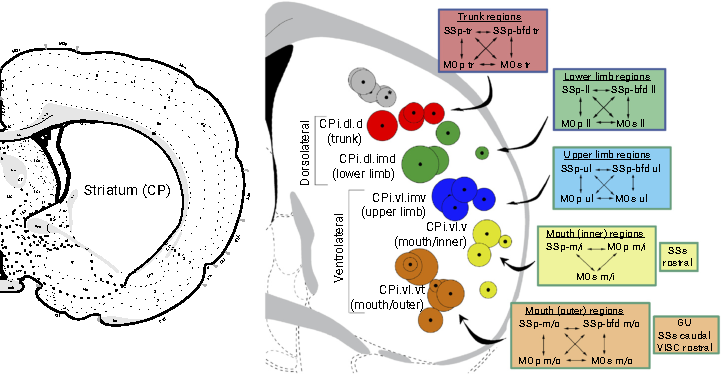
\includegraphics[width=0.9\linewidth]{ch-intro/figures/StriatumInputMap}
    \caption[Somatotopic map of cortical inputs to \gls{dls}]
    {\textbf{Somatotopic map of cortical inputs to \gls{dls}.}
    \textit{Left}: striatum in the rat brain atlas.
    \textit{Right}: input from somatosensory cortices form a topographic map in the \gls{dls}.
    Abbreviations are defined in the original reference and are not important for the purposes of this work.
    Figure adopted from~\cite{Hintiryan2016NN}.
    }
    \label{fig:intro:InputMap}
  \end{center}
\end{figure}
Of note, \gls{dms} and \gls{dls} have been suggested as functionally distinct areas as well, contributing to goal-directed and habitual behaviors, respectively~\cite{Yin2006NatRevNeurosci}.
Another noteworthy result concerns the extent of these areas.
The identified \gls{dls} receives inputs from motor cortex, somatosensory cortex, but also frontal association cortex, amygdala, and prelimbic cortex, and expands medially much larger than what has been traditionally regarded as \gls{dls}.
It has since been suggested that the sensorimotor information in the dorsal striatum is more prevalent than classically considered and it should be taken into account in studies concerning the function of the striatum~\cite{Robbe2018}.


\subsubsection{Direct/Indirect Pathways}
\label{intro:bg:pathways}
\Glspl{msn} are the majority of the neuronal population of the striatum.
They are homogeneously distributed in a way that the striatum lacks any architectural organization when all the neurons are stained in a histologic slice~\cite{Dudman2015Book}.
Nonetheless, \glspl{msn} are divided into two major categories, based on their neurochemistry and connectivity.
One class expresses \gls{d1} and projects directly to \gls{gpi}/\gls{snr} neurons, hence they form the so-called \emph{direct pathway}.
The second kind expresses \gls{d2} and projects to the \gls{gpe}.
This pathway, in turn, leads to the output nuclei through two routes:~monosynaptic~\gls{gpe}$\rightarrow$output, or bisynaptic~\gls{gpe}$\rightarrow$\gls{stn}$\rightarrow$output projections~\cite{TURNER2000BasalFunction}.
These \glspl{msn} form the \emph{indirect pathway}~(\autoref{fig:intro:BGAnatomy}).
\Gls{d1}-expressing neurons and \gls{d2}-expressing neurons exist in rather equal numbers and are intermingled and spread rather uniformly throughout the striatum~\cite{Dudman2015Book}.
The net effect of direct pathway activity is to inhibit the \gls{gpi}/\gls{snr}, thus releasing the target areas of the \gls{bg} from inhibition.
On the contrary, indirect pathway activity, through \gls{gpe} and \gls{stn}, disinhibits the output nuclei that in turn would cause further inhibition of \gls{bg} targets.
\par
\Gls{da} significantly modulates neuronal activity in the striatum.
\Gls{pd}, with many behavioral and cognitive ramifications, is characterized by degeneration of \gls{snc} neurons and \gls{da} depletion in the striatum~\cite[see][for a comprehensive review]{McGregor2019Neuron}.
Axons from \gls{snc} neurons arborize widely in the striatum.
They primarily synapse with principle neurons (\glspl{msn}), targeting the narrow necks connecting the spines to dendritic shafts, whereas cortical inputs mostly terminate on dendritic shafts.
This particular arrangement may be a mechanism by which \gls{da} release modulates cortical input to the \glspl{msn}~\cite{TURNER2000BasalFunction}.
This mechanism is of extra importance since \gls{d1}-expressing neurons are excited by \gls{da}, whereas \gls{d2} neurons are inhibited.
Thus \gls{da} signals can up-regulate or down-regulate the excitability of the direct and indirect pathways.



%============================================================
\subsection{Basal Ganglia as a Clock}
\label{ch:intro:BGTime}

Many brain structures have been proposed to contribute to time estimation.
Among them, the \gls{bg}, are especially of interest, since they are directly involved in motor processes as well~\cite{Grillner2015}.
Moreover, the \gls{bg} are also involved in reinforcement learning---selecting actions in an uncertain world in a way that maximizes reward in the long term~\cite{Petter2018}.
Such learning necessitates an understanding of temporal contingencies in order to maximize future rewards.
Behavioral data supports that animals build probabilistic models for timing of the reward and even adjust their models in response to modified reward delays~\cite{li2013PNAS}.
% In general, execution of any complex behavior requires proper timing of the comprising sub-actions.
\par
The \gls{bg} are often implicated in timescales of several hundreds of milliseconds to several seconds~\cite{Paton2018NeuronRev}.
Evidence of involvement of the \gls{bg} in timing stems from a variety of sources, including pathologies such as \gls{pd}, lesion studies, and pharmacological and genetic manipulations.
Following the taxonomy discussed in \autoref{ch:intro:taxonomy}, there is some evidence of involvement of the \gls{bg} in sensory timing.
\Citeauthor*{Rao2001} reported encoding of time intervals in the human striatum in a task in which subjects reported whether an interval were shorter or longer than a standard interval of 1200~ms.\footnotemark\
They also observed a dynamic network of cortical activity in inferior parietal, premotor, and dorsolateral prefrontal cortex.
These nodes in the network were attributed to different components of temporal processing, respectively, attention, memory, and interval comparison.
They ultimately concluded the implication of ``striatal dopaminergic neurotransmission in hypothetical internal timekeeping mechanisms"~\cite{Rao2001}.
\footnotetext{
    This paradigm is commonly referred to as ``interval categorization task".
    }
Moreover, \Citeauthor*{Pouthas2005} investigated interval categorization for two durations (450~ms and 1300~ms).
They observed ramping striatal activity during both intervals.
They concluded a direct role of the basal ganglia in duration estimation, and that the caudate nucleus ``may support a clock mechanism"~\cite{Pouthas2005}.
Similar evidence exists in other species as well.
\Citeauthor*{Gouvea2015Elife} trained rats in a sensory categorization task to judge whether an interval is shorter or longer than 1.5~s.
They decoded animals' choice and elapsed time from ensembles of striatal neuronal activity, whereas apparent behavior in an overhead video failed to do so.
Importantly, transient inactivation of the \gls{ds} impaired performance, however, it did not cause a systematic under-- or over--estimation~\cite{Gouvea2015Elife}.
\par
Furthermore, the \gls{bg} are also well studied for their role in motor timing.
\Citeauthor*{Matell2003} trained rats to receive a reward in a fixed interval reinforcement schedule.\footnotemark\
The interval alternated between 10~s (25\% of trials) and 40~s (75\% of trials).
After learning, animals increased their lever press rate around the reinforced intervals.
Electrophysiological recordings from the striatum showed neurons with tuned firing rate only around 10~s interval, but not 40~s, while apparent behavior of the animals is similar.
The authors then suggest that a population of duration-coding cells, each tune to different values, could accurately represent the elapsed time~\cite{Matell2003}.
\footnotetext{
    In operant conditioning, fixed interval reinforcement schedule refers to a type of conditioning whereby a response is reinforced only if a certain period of time has elapsed.
    }
\Citeauthor*{Mello2015} also used a similar task for intervals ranging between 12~s to 60~s.
They found striatal cells that rescaled their activity when intervals changed.
As rats adjusted to the new interval, time estimations decoded form population dynamics predicted animals' timing performance.
In another study, \Citeauthor*{Bakhurin2017JNeuro} used an operant conditioning paradigm in which the conditioned stimulus was followed by a delayed reward delivery (2.5~s after cue onset) and they monitored anticipatory licking of mice as behavioral readout of temporal perception.
After training, they started licking~$\sim$1.5~s after the conditioned stimulus.
Simultaneously recorded neurons in the striatum and orbitofrontal cortex displayed sequential activity during the interval.
A machine learning algorithm was then trained to decode the elapsed time from the stimulus onset.
They showed that both striatal and cortical networks ``encoded time, but the striatal network outperformed the orbitofrontal cortex".
Interestingly, removing the neurons modulated by licking activity from the decoder significantly reduced its performance, however, it still remained higher than chance level~\cite{Bakhurin2017JNeuro}.
\par
Another source of impact in the \glsentrylong{bg} is the neuromodulatory effect of \gls{da}.
\Glsentrylong{da}'s role in reward processing and circuit dynamics of the striatum is discussed in \autoref{intro:BGAnatomy} and \autoref{intro:BGMotor}.
\Gls{da} is also believed to be involved in timing~\cite{Paton2018NeuronRev}.
In a peak interval procedure\footnotemark, \Citeauthor*{DeCorte2019} found that \gls{d2} blockade delayed start and stop times for an interval of 6~s.
Whereas, blockade of \glspl{d1} delayed stop times only.
Then they stressed the role of the \gls{ds} in timing, with \gls{da} ``being particularly critical for the temporal control of action"~\cite{DeCorte2019}.
\footnotetext{
    Peak interval procedure is a common task used to study timing.
    Similar to fixed interval schedules, a cue indicates that a response will be reinforced only after a certain period of time has elapsed.
    The profile of the response around the interval is then studied.
    }
\Glsentrylong{da} neurons encode reward prediction errors which requires accurate reward predictions~\cite[see][]{Berke2018NN}.
\Citeauthor*{Takahashi2016} recorded from \gls{da} neurons of rats while they performed a task with uncertainty in reward timing and reward number.
Neuronal activity showed error signals in response to both types of prediction error, however, after ventral striatal lesions, neurons only responded to changes in reward number, and not reward timing.
These results suggested that time-dependant component of reward prediction of \gls{da} neurons might rely on the ventral striatum~\cite{Takahashi2016}.
In an interesting study, \Citeauthor*{Paton2016Sci} measured and manipulated the activity of \gls{da} neurons in a 1.5~s interval categorization task.
\Gls{da}ergic activity predicted animal's time estimates.
Transient activation/inhibition of \gls{da} neurons caused under--/over--estimation of the interval.
Hence, they concluded that ``\gls{da} neurons, which are so central to reward processing, exert control over time estimation"~\cite{Paton2016Sci}, although these results reflect \gls{da} function in general, not specifically in the \gls{bg}.
Similar to scaling of spiking activity in the striatum~\cite{Mello2015}, \gls{da} concentration in the \gls{ds} is also scalable to time intervals in several second time range~\cite{Howard2017}.
However, \citeauthor{Howard2017} then conducted a series of experiments and concluded that the \gls{da} signal in the \gls{ds} does not reflect interval timing per~se, rather it is specific to behavioral choice of action~\cite{Howard2017}.
\par
Deficits in temporal perception occur in many disorders.
Since pathologies usually affect multiple brain structures or manifest in several behavioral domains, it is unclear whether timing deficits are responsible for dysfunctions, or they are merely the result of other malfunctioning systems.
Schizophrenia, for example, is a complex psychiatric disorder with a wide range of symptoms, including: delusions, hallucinations, speech poverty, and timing deficits.
This impairment is reported in sensory and motor timing tasks and is associated with increased \gls{da} levels in the striatum, as well as abnormal activity in the dorsolateral prefrontal cortex and \gls{sma}~\cite[see][]{Snowden2019}.
Furthermore, it has been reported that individuals with attention deficit/hyperactivity disorder do not benefit from temporal predictabilities in an oculomotor task that displayed a target after a random delay~\cite{Dankner2017}.
Additionally, timing deficiency has also been reported in \gls{hd}.
Patients demonstrated lower sensitivity to temporal regularities and overall, poorer performance in different types of sensory timing tasks.
Their performance negatively correlated with the progression of the \gls{hd}~\cite{Cope2014}.
Finally, \gls{pd} also affects timing performance.
Lower timing performance has been reported in multiple tasks.
\Citeauthor*{Harrington1998} showed that \gls{pd} patients were impaired in sensory timing, in which `duration perception' was weaker compared to the control group.
Also, in a motor task, whereby subjects performed finger-tapping synchronized with a series of tones (in the subsecond range), \gls{pd} participants were significantly more variable~\cite{Harrington1998}.
Interestingly, it has been proposed that frequent exposure temporally-structured tones might alleviate motor symptoms of the \gls{pd}, especially gait and stride length~\cite{Dalla2017}.

%============================================================
\subsection{Basal Ganglia as a Cost Machine}
\label{intro:BGMotor}
\epigraph{Why do we and other animals have brains?\dots You may reason that we have one to perceive the world or to think, and that is completely wrong\dots We have a brain for one reason and one reason only, and that is to produce adaptable and complex movements.}
{\textit{Daniel Wolpert, TED talk}}
\noindent

Regardless of whether one agrees with Daniel Wolpert's strong words above, importance of volitional movement is trivial.
Control of movements has been associated with \gls{bg} for a long time.
This link dates back to the first descriptions of the behavioral deficits of \gls{pd} by James Parkinson in 1817.
% \Gls{pd} is characterized by loss of \gls{snc} neurons and their ascending projections to the striatum.
Tetriakoff, in 1919, performed postmortem analysis of the brains of patients diagnosed with \gls{pd} and first reported loss of dark-pigmented nigral neurons.
Ever since, motor dysfunctions of \gls{pd} are believed to be due to \gls{da} depletion in the striatum~\cite{Hornykiewicz2006,McGregor2019Neuron,Redgrave2010}.
\par
Three behavioral deficits are typical for \gls{pd} (although symptoms differ from patient to patient):
    1)~resting tremor, which is the most apparent;
    2)~rigidity and stiffness of muscles;
    3)~bradykinesia---reduced movement vigor.
Reduced vigor in \gls{pd} has been investigated to distinguish between speed-accuracy trade-off and energetic cost as two possible determinants of movement speed.
\Citeauthor{Mazzoni2007} asked \gls{pd} patients and age-matched control subjects to make self-paced arm movements as accurate as possible toward a target with a speed within the requested range~\cite{Mazzoni2007}.
After 20 successful trials, the required speed range and/or target distance changed to the next experimental condition.
Both groups of subjects, across all conditions (3~target distances, 4~speed ranges) achieved similar peak velocities and maintained the same level of accuracy.
However, patients needed significantly more trials to reach the criterion to advance to the next condition.
Analysis of those extra trials performed by the \gls{pd} patients demonstrated that they used a higher proportion of slower movements while retaining the speed range the same as control subjects.
Moreover, authors showed that the number of trials required to reach the criterion, as a measure of task difficulty, strongly correlated with subjects' average acceleration.
This linear contribution (denoted as $S_N$) was steeper for control subjects.
In other words, for any given difficulty of the task, \gls{pd} patients \textit{chose} a lower level of acceleration.
Similar linear relationship existed between number of trials to criterion and accuracy as well, but it was the same for control subjects and patient.
Thus, lower $S_N$ in \gls{pd} is not caused by a different speed-accuracy trade-off, rather another component of task difficulty related to the acceleration.
Authors then argue that acceleration also represents movement energy cost, and that \gls{pd} patients are more sensitive to energy expenditure.
These results suggest that \gls{snc} innervation of the striatum carries a `motor motivation' signal and lack thereof in \gls{pd} leads to a propensity for slow movements~\cite{Mazzoni2007}.
\par
Available methods in animal research provide an opportunity to further dissect the \gls{bg} circuits.
For instance, infusion of the GABA$_A$ agonist, muscimol, transiently inactivates the surrounding neurons, allowing the researcher to study the functional relevance of the targeted structure.\footnotemark
\Citeauthor{Desmurget2010JNeurosci} took advantage of this technique to acutely inactivate the sensorimotor territory of the \gls{gpi} in monkeys~\cite{Desmurget2010JNeurosci}.
The monkeys were trained to move a cursor using a joystick to a peripheral target and then it back to its original position.
Two experimental conditions differ in the degree to which successive target positions were predictable:
    random positioning of the target in each trial;
    or a fix sequence of four target positions.
\Gls{gpi} inactivation after overlearning the sequence did not prevent its execution, thus failing to support a role for the \gls{bg} in ``storage or execution of well learned motor habits".
The main impairment observed post-injection was reduced movement speed and amplitude in both conditions, i.e., random sequences and the overlearned sequence.
Thus, they conclude that the motor circuit of the \gls{bg} contributes to the kinematics of motor execution but not its production nor storage of learned sequences~\cite{Desmurget2010JNeurosci}.
\footnotetext{
    This technical approach is not free from skepticism.
    \Citeauthor{Otchy2015Nature} present convincing evidence that acute circuit manipulations, such as inactivation, have unintended consequences.
    In a complex dynamical system such as the brain, by transiently changing the activity of the area of interest, off-target down-stream structures are driven into a unnatural state that could have behavioral implications of its own~\cite{Otchy2015Nature}.
    }
Similar results have been reported from patients with pallidal and striatopallidal lesions.
They can generate normal grip force when explicitly instructed, however once left to their own, they fail to squeeze harder to earn more monetary compensation~\cite{Schmidt2008Brain}.
In general, reduced vigor in common in conditions of abnormal \gls{bg} function~\cite{}.
Importantly, in many of those tasks, including the two mentioned above, reduced vigor could also be the consequence of overestimation of the cost.




% 1- vigor reduction is very common
% 2- in most tasks, vigor reduction translates to energetic conservatism
\section[Motivation, Question and More]{Motivation, Question and the Organization of the Thesis}
\label{intro:question}

The work presented in this thesis has two fronts that might seem unrelated at first glance, but in this chapter I tried to present them on a conceptual continuum.
The first part is concerned with the question of how animals often act as though they have a sense of time.
Enormous body of experimental and theoretical research implicates plenty of brain areas as providers of a time signal.
Although such an internal mechanism could be affected by external factors (e.g., reward rate and motivation), however it is usually assumed to be the means by which well-timed actions are generated.
This is what I referred to as ``internal time estimation'', not that the world exterior to the brain is irrelevant, but meaning that the brain has a sense of time on its own that underlies behavior.
This mechanism is appealingly simple, predictive of many behavioral phenomena, and backed by neurophysiological data.
Alternatively, we hypothesized that there is no sense of time per~se, and that time is perceived through interactions with the environment.
In other words, the duration of an interval is displaced by its sensorimotor content.
Since movement generation is among the most basic functions of the nervous system and inevitably, it takes a certain duration to execute any action, elapsed time could just be inferred from actions (or similarly, sensory processes).
Such an ``embodied time estimation'' provides a much more parsimonious explanation, and is in alignment with the long-reported and replicated observation across many species that animals produce stereotyped motor sequences under temporal constraints.
Nonetheless, this hypothesis has not been very popular!
Perhaps partly due to technological limitations to monitor a wide range of animal behavior (in rodents, from locomotion to whisking and sniffing), especially in standard experimental paradigms inside Skinner boxes; and in my opinion, partly due to a general brain-centric view where the brain is the puppeteer of the body.
\par
To test the embodied timing hypothesis, we used a novel behavioral paradigm developed by~\citeauthor{Rueda2015NN}~\cite{Rueda2015NN} that is a powered treadmill with a reward contingent on timing of appetitive approaches (details are discussed in \autoref{ch:methods:methods}).
This task allows monitoring the location of the animals and kinematics of their locomotion.
Powered treadmill enabled us to manipulate dynamics of the environment in order to facilitate or hinder exploitation of the stereotyped motor sequences that we hypothesized are essential for solving the task.
We assumed if timing was internally-driven, animals should be able to perform the task without resorting to the stereotyped motor strategies.
Results from these experiments are presented in \autoref{ch:time}.
\par
The second facet of this work deals with the problem of implementation, i.e., how the brain generates the motor 
sequence it presumably uses to keep track of time.
Classic models of the \gls{bg} implicate the \gls{dms} in early phases of learning, and the \gls{dls} in executing the learned sequences, or controlling their kinematics.
Results from an earlier work in our group suggest that the overall behavior of the animals following transient inactivation of the \gls{dls} remains intact, although more variable~\cite{Rueda2015NN}.
Therefore, in this work, using a similar approach, we aimed to specify the function of the striatum in development and execution of this behavior.
In particular, we evaluated the role of the striatum, the main input to the \gls{bg}, in learning and controlling the kinematics of a motor sequence, by permanently lesioning its subareas (details are discussed in \autoref{ch:methods:tech}) in both na\"{i}ve and trained animals.
Results from these experiments are presented in \autoref{ch:lesion}.
\par
Finally in \autoref{ch:discussion}, I synthesize an overview of my Ph.D.\ project and discuss its meaning and implications.
Moreover, some possible shortcomings and directions for future works are laid out.
It also should be noted that I tried to write each chapter such that it would make sense on its own, regardless of the rest of the manuscript.